
\chapter{提案}
\label{chap:suggestion}

この章では、ARを用いた生活の簡素化支援システムについて提案し、その具体的な用途について、各例ごとに考察する。

\newpage

\section{ARを用いたモノの仮想的代替による簡素化支援システムの提案}
\label{chap:suggestionDetail}

\subsection{概要}

簡素化支援システムとは、生活の簡素化のために排除したモノをARで仮想的に再現し、その代替として利用することで、簡素化前と同程度、或いはそれ以上に充実した機能を得ることができる、実世界の一部を代替するインターフェースである。

なお、ARでの仮想的な代替を実現するため、常にARデバイスを使用し続ける事を前提としている。

\subsection{仮想的な代替が可能なモノ}

モノの中には、仮想的な代替が可能なモノと不可能なモノが存在する。人や物体の支えとなるモノや、温度を制御する機能を持つモノなど、対象のモノがその場になくては役割を果たせないものか否かで判別する。下記の表は、一般的な部屋内のモノについて、その場になくても役割を果すものとそうでないものを分類したものである。

\begin{table}[htbp]
    \caption{その場になくては役割を果たせないものか否か}
    \label{tb:mono}
    \begin{center}\begin{tabular}{c|c}
      \hline
      なくてはならないもの&机・椅子・本棚・タンス・冷蔵庫・洗濯機・エアコン etc.\\\hline
      なくてもよいもの&テレビ・時計・PCディスプレイ・カレンダー・ポスター etc.\\\hline
    \end{tabular}\end{center}
\end{table}

簡素化支援システムでは、後者に分類されたモノを実世界で配置する代わりに、ARを用いて仮想的に表示することにより、生活の機能充実を損なわずに、実世界の空間の簡素化を実現する。

\subsection{使用するARデバイスについて}
\label{chap:ARdevice}

簡素化支援システムは、日常的に利用される前提のため、デバイスについても同様に日常的に使用できることが条件となる。現段階では、ARグラスがその条件を満たす技術であると推察する。ARグラスとは、実世界に重ねて描画できるグラフィックデバイスで、実世界を認識して得た情報を元に、実世界に重ねて表示をする眼鏡型のデバイスである。代表的なARグラスとして、Hololens\footnote{Microsoft Hololens: \url{https://www.microsoft.com/ja-jp/hololens}(accessed 2021-01-26)}、Magic leap 1\footnote{Magic leap 1: \url{https://www.magicleap.com/ja-jp/magic-leap-1} (accessed 2021-01-26)}、Nreal light\footnote{Nreal light: \url{https://www.nreal.ai/light/} (accessed 2021-01-26)}などがある。いずれもPCを必要とせず、スタンドアロンで動作する。空間に対する位置・角度などを検知できるため、6DoF(six degrees of freedom)に対応しており、高い没入感を得ることができる。

\newpage

\section{簡素化支援システムの具体的なシナリオの考察}

ここでは、\ref{chap:suggestionDetail}にて挙げた生活の簡素化支援システムについて、より具体的なシナリオを交えた上で、多角的に考察する。

\subsection{部屋の空間の確保と機能性の拡張}

\ref{tb:mono}で提示したモノを部屋から排除することにより、実世界に空間を確保をすることができる。確保した空間には、ARで再現したモノを表示するが、状況に応じて非表示にしたり、別のモノを表示することも可能なため、より自由度の高い空間として利用することが可能である。また、ARによって仮想的に表示しているため、物理法則に囚われない表示をすることも可能である。壁や天井などは使用されていないスペースとなっている場合が多いが、そういったスペースも有効活用できる。

また、実際には配置することが難しいモノを配置することで、部屋内の機能をより充実させることができる。例えば、スマホウィジットに代表される、時間、天気やカレンダー、todo、体調状態、メモなどを配置することで、スマートフォンのホーム画面のように使用できる(図\ref{fig:widget})。なお、スマートフォンでの時刻や日付の確認が容易になった現代でも、カレンダーや時計を部屋に配置する事と同様に、これらの情報を実世界上で見られるようにすることで、モノの位置を、部屋内の絶対位置やモノ同士の相対的な位置関係といった二次的な情報に紐づけて記憶することができ、欲しい情報を瞬時に獲得、もしくは機能を利用する事ができるのではないかと推察する。

\begin{figure}[htbp]
    \begin{center}
       \fbox{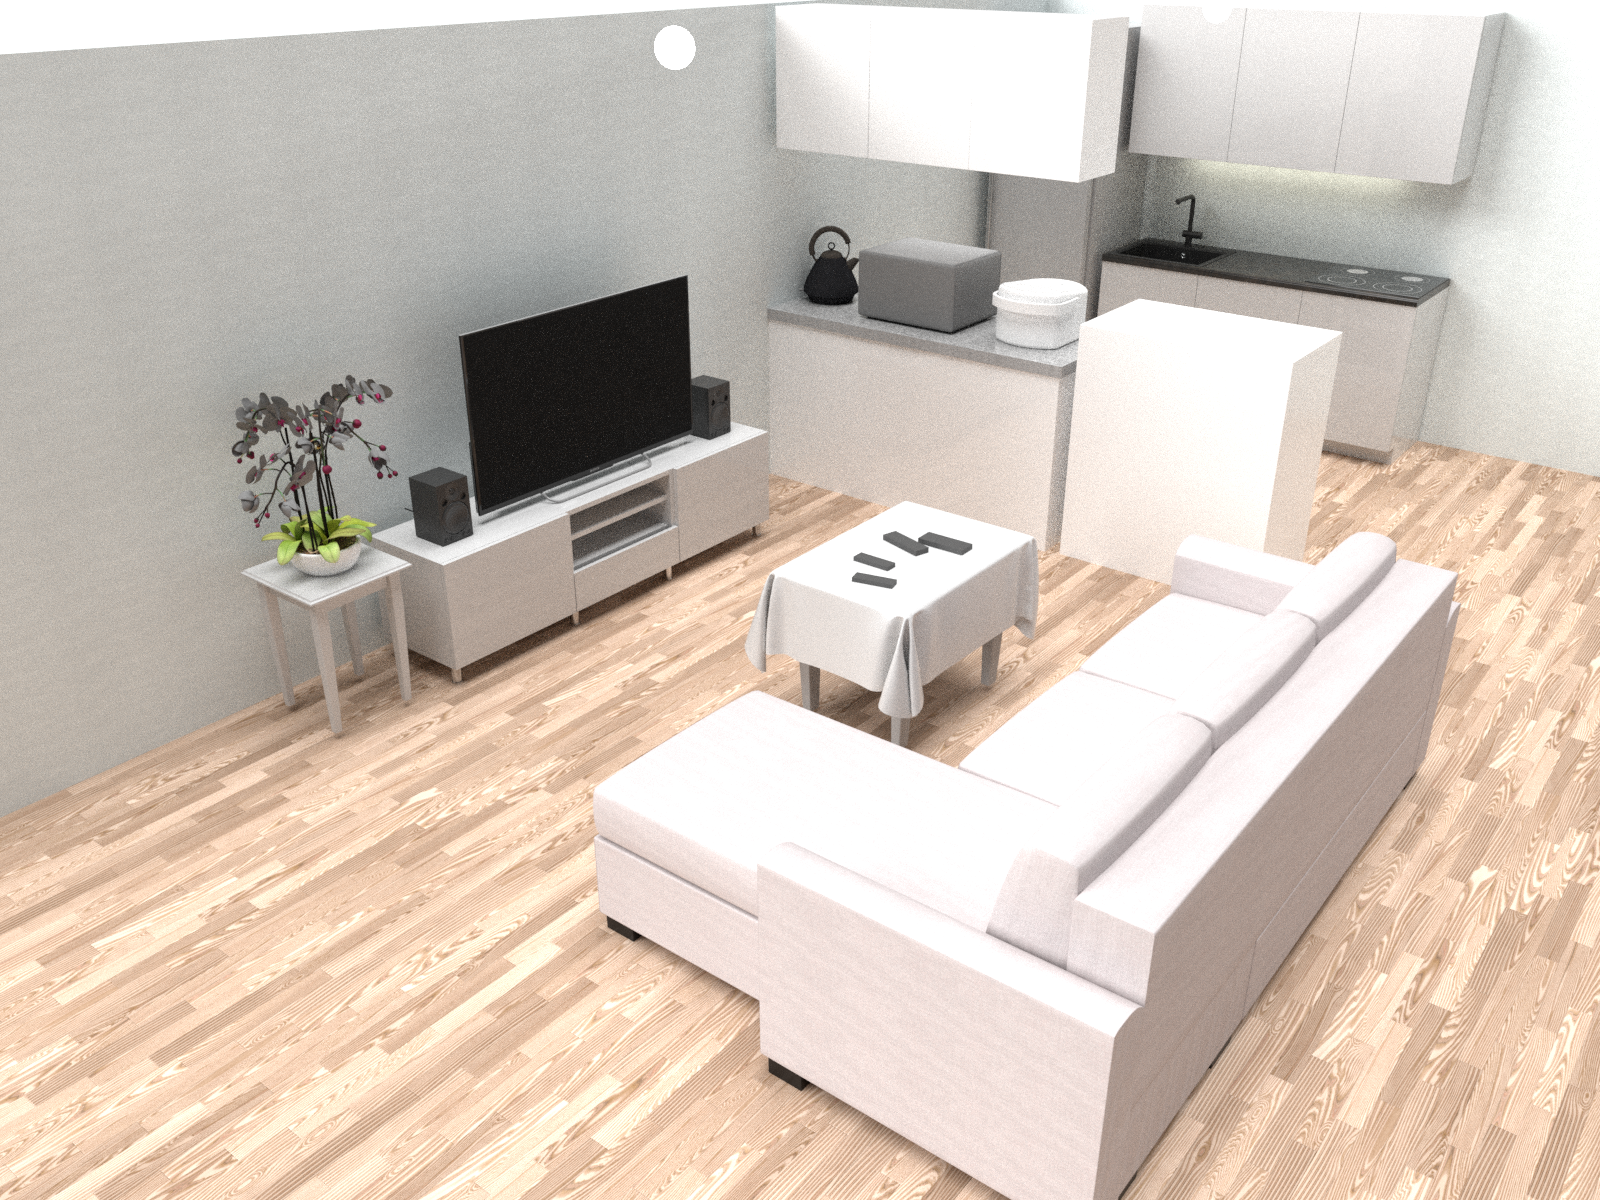
\includegraphics[width=60mm]{images/living_room_01.png}}
    \end{center}
    \caption{通常の部屋環境のイメージ}
    \label{fig:normal-room}
\end{figure}

\begin{figure}[htbp]
    \begin{minipage}{0.5\hsize}
      \begin{center}
        \fbox{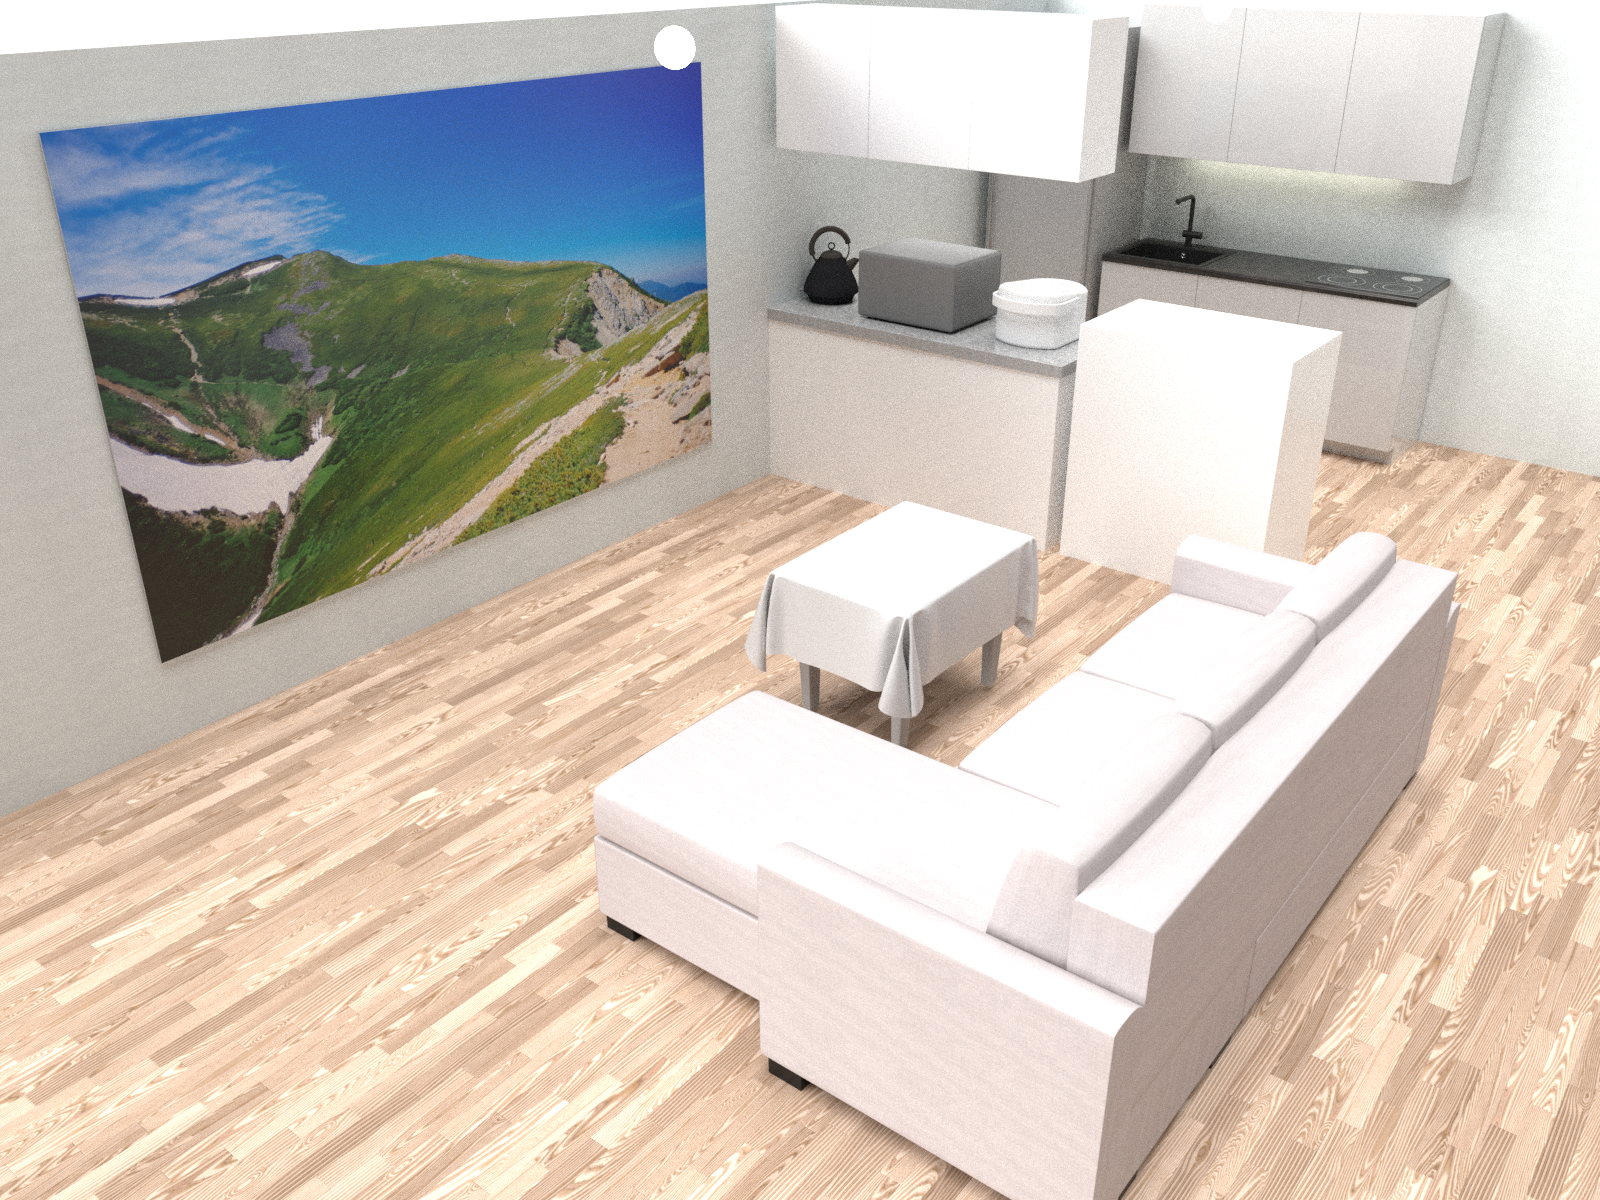
\includegraphics[width=60mm]{images/living_room_02.png}}
      \end{center}
      \label{fig:bigTV}
      \caption{テレビを仮想的に代替したイメージ}
    \end{minipage}
    \begin{minipage}{0.5\hsize}
      \begin{center}
        \fbox{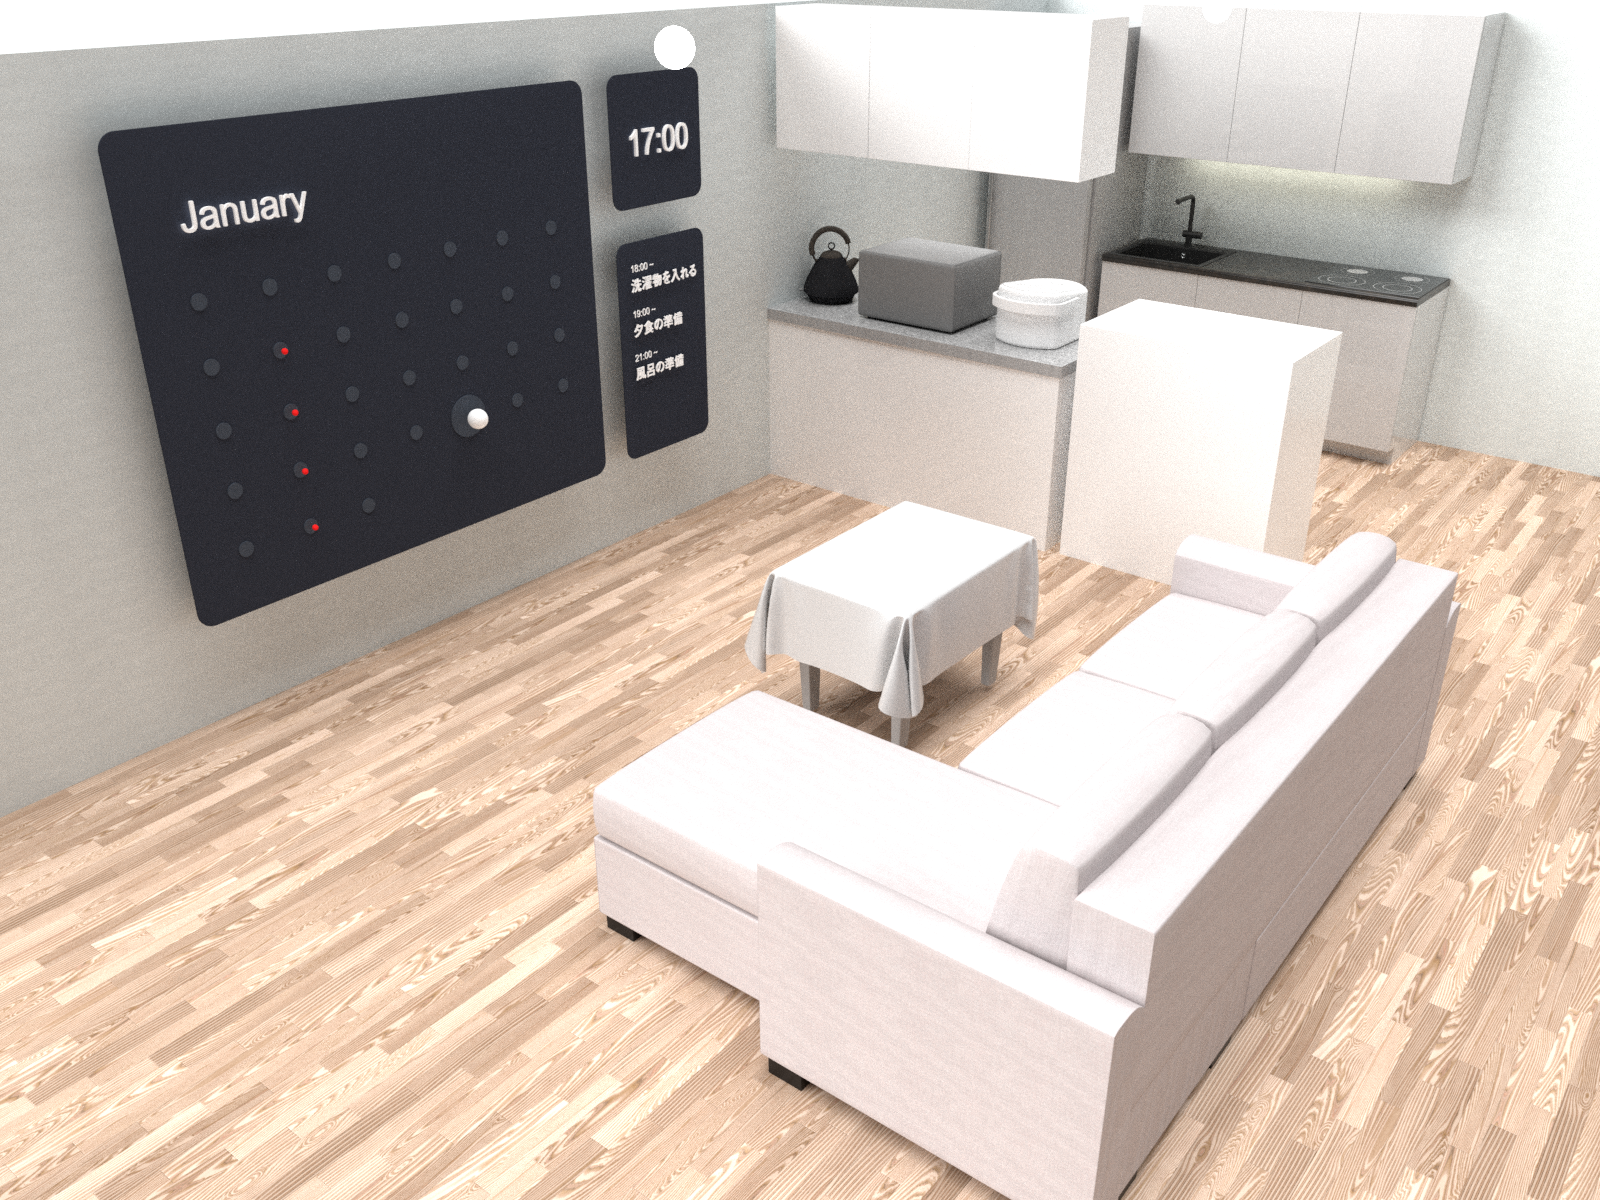
\includegraphics[width=60mm]{images/living_room_03.png}}
      \end{center}
      \caption{部屋をスマホのホーム画面のように使用できるイメージ}
      \label{fig:widget}
    \end{minipage}
\end{figure}


\subsection{同様の環境を他所で再現}

自身が身を置く場所は常に一定ではなく、自宅の部屋以外にもオフィスやカフェ、ホテルなどの場所に身を置くこともある。その際に、本システムを利用する事で、普段とは違う場所でも自室の環境を再現することができる。

また、他所の部屋環境を自身の部屋環境として再現することも可能である。オフィスや映画館など、シチュエーションに応じたモノの再現が可能なため、より個人の充実に適した環境を用意することができる。

\subsection{物体の管理や更新、カスタマイズ}

仮想的なモノは実体を持たないので、購入や修理などのコストがかからない。また、物体の更新にも物理的なコストは掛からないので、色や形、大きさまで、自由にカスタマイズすることができる。

